\documentclass[conference,letterpaper]{IEEEtran}
\IEEEoverridecommandlockouts

% Arabic decimal section numbering (1, 2, 2.1, 3.3) instead of IEEEtran's
% default Roman-numeral/letter scheme (I, IV-A). Both \ref-facing counters
% and the visible heading forms are redefined so headings and every \ref
% call render identically -- these are the same definitions IEEEtran.cls
% itself uses under its \texttt{compsoc} class option, adopted directly
% here without invoking \texttt{compsoc} itself, which changes fonts and
% spacing project-wide.
\renewcommand{\thesection}{\arabic{section}}
\renewcommand{\thesubsection}{\thesection.\arabic{subsection}}
\renewcommand{\thesubsubsection}{\thesubsection.\arabic{subsubsection}}
\renewcommand{\theparagraph}{\thesubsubsection.\arabic{paragraph}}
\renewcommand{\thesectiondis}{\thesection}
\renewcommand{\thesubsectiondis}{\thesubsection}
\renewcommand{\thesubsubsectiondis}{\thesubsubsection}
\renewcommand{\theparagraphdis}{\theparagraph}

\usepackage{cite}
\usepackage{amsmath}
\usepackage{amssymb}
\usepackage{graphicx}
\usepackage{textcomp}
\usepackage{xcolor}
\usepackage{booktabs}
\usepackage{multirow}
\usepackage{tabularx}
% float's [H] specifier (used on Tables II and IV): pins a table to its
% exact source position instead of IEEEtran's normal top-of-column float
% heuristic, which was landing both tables at the top of whichever column
% happened to break nearest their declaration -- sometimes *before* the
% very subsection heading that introduces them in reading order, not
% after it as the source order intends.
\usepackage{float}
\usepackage[hidelinks]{hyperref}

\graphicspath{{figures/}{../analysis/figures/}}

% Every quantitative value cited in the results/discussion is a \NumXXX
% macro defined here, read live from analysis/*.csv by
% scripts/build_paper_values.py -- never hand-type a result value in a
% sections/*.tex file. Regenerate with `make values` before compiling if
% analysis/ data has changed since this file was last generated.
\input{values}

\def\BibTeX{{\rm B\kern-.05em{\sc i\kern-.025em b}\kern-.08em
    T\kern-.1667em\lower.7ex\hbox{E}\kern-.125emX}}

% Reclaim the dead band between the title block and the body text.
% IEEEtran reserves a fixed spacer there and quantizes it to a whole
% \baselineskip so body baselines align on a grid (\IEEEquantizevspace,
% called from \maketitle); \@IEEENORMtitlevspace/\@IEEEMINtitlevspace are
% its nominal and floor values (1 and 0.75\baselineskip under the
% conference option). With every front-matter line folded into \title{}
% and \author{} left empty, that spacer plus the empty author block left
% a 55.5pt band of white on page 2 -- about 4.6 lines of body text --
% measured 2026-09-02. Note a plain \vspace after \maketitle cannot
% remove it: that glue lands at the top of column 1 and TeX discards
% glue at the top of a column (which is why the pre-existing
% \vspace{-30pt} below has no measurable effect at any value).
% Zeroing these two, plus the \vspace at the end of \title{}, cuts the
% band to 8pt. That matters beyond page 2: the space it frees is what
% allowed the four \enlargethispage calls in sections/ -- which bought
% room by pushing text *below* the bottom margin -- to be halved.
\makeatletter
\def\@IEEENORMtitlevspace{0pt}
\def\@IEEEMINtitlevspace{0pt}
\makeatother

% Space between a float and the text below it. IEEEtran's default is
% 18.6pt plus 2.4 minus 4.8; combined with the 12pt skip a \subsection
% adds before its heading, a figure sitting at the top of a column and
% followed by a heading (Figure 2 into Section 4.6) opened a 45pt hole --
% and because \flushbottom fills a column by stretching whatever glue it
% can find, the column's leftover space was landing in that one gap
% rather than spreading out. Measured 2026-09-02: 45.1pt from the Figure 2
% caption to the 4.6 heading. Trimming this to 12pt closes it and, by
% freeing space document-wide, also removed the last bottom-margin
% overrun on the reference page. Adding \parskip stretch was tried as an
% alternative (to spread the slack across paragraph breaks instead) and
% did not help -- the gap stayed at 44.6pt.
\setlength{\textfloatsep}{12pt plus 2pt minus 4pt}

\begin{document}

% Declaration + Acknowledgment moved to the very front, per explicit
% instruction: this is now the document's first page, the actual paper's
% title page its second. \onecolumn here (IEEEtran conference is
% twocolumn from \begin{document} by default) renders the cover-sheet
% scan at full page width; \twocolumn below switches back before
% \maketitle. Both switches force their own page break on their own, so
% neither end of this block needs an explicit \clearpage/\newpage.
% ---------------------------------------------------------------------
% PAGE 1: the degree title page. A title page is a page -- this content
% used to sit in the \title{} block of the paper's own first page, where
% it displaced the IEEE author block. It is single-column, centred, and
% carries no page number, no abstract, no keywords and no acknowledgment.
% \onecolumn (IEEEtran conference is twocolumn from \begin{document}) is
% what makes it full-width; it forces its own page break, so nothing
% before it needs a \clearpage.
% ---------------------------------------------------------------------
\onecolumn
\thispagestyle{empty}
\begin{center}
\vspace*{0.14\textheight}

{\LARGE Dynamic, Template-Based Benchmarking Resists\\[0.35em]
Contamination-Induced Score Inflation in LLM\\[0.35em]
Unit-Test Generation\par}

\vspace{0.10\textheight}

{\large
A dissertation submitted in partial fulfilment of\\[0.30em]
The requirement for the degree of\\[0.30em]
MASTER OF SCIENCE in Artificial Intelligence\\[0.30em]
in\\[0.30em]
The Queen's University of Belfast\\[0.30em]
By\\[0.30em]
Yohan Sneider Sanchez Vega\\[0.30em]
03/09/2026\par}
\end{center}
\clearpage

% ---------------------------------------------------------------------
% PAGE 2: the signed declaration cover sheet, plus the acknowledgment,
% which stays here rather than moving to the title page. Still
% single-column; \twocolumn below switches back for the paper itself and
% forces its own page break.
% ---------------------------------------------------------------------
\thispagestyle{empty}
\begin{center}
\vspace*{-24pt}
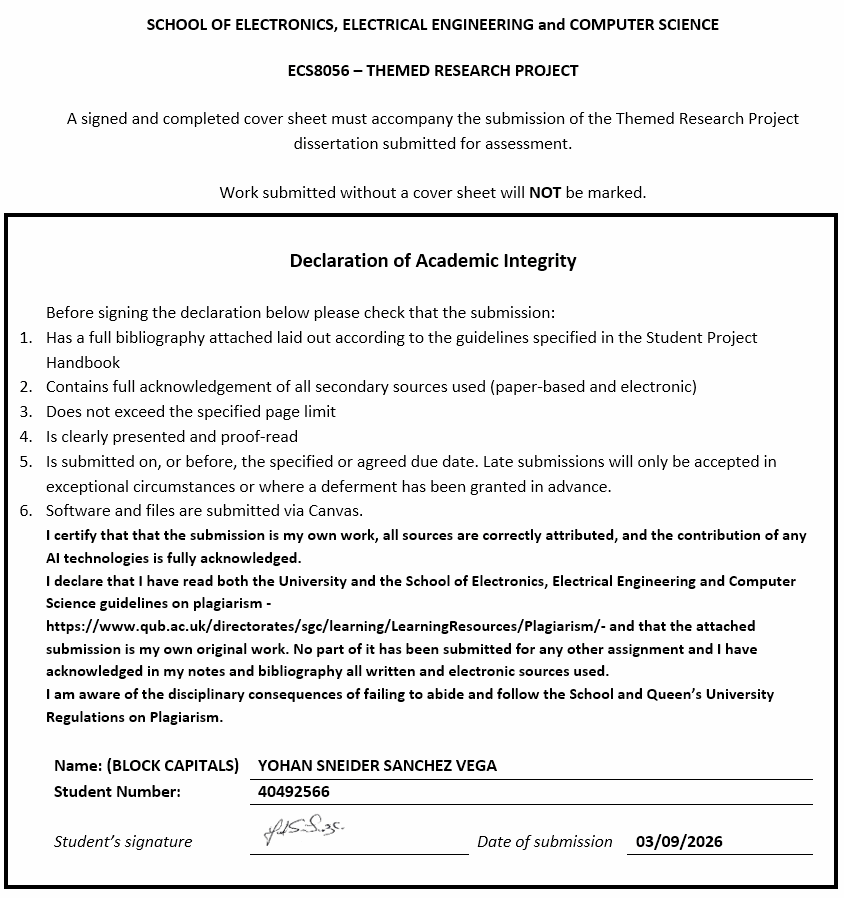
\includegraphics[width=0.97\textwidth]{Declaration_2.png}
\end{center}
\noindent{\bfseries\MakeUppercase{Acknowledgment}}\par\medskip
\noindent The author would like to thank Dr Pinzhen Chen for his guidance throughout this project, all the professors who shared their knowledge during the course, and the Northern Ireland High Performance Computing (NI-HPC) service for the computing resources.

\twocolumn

% The paper's own first page: title, then the standard IEEE author block.
% The degree statement that used to live inside \title{} here has moved to
% the standalone title page (page 1) -- it is not a title block, and
% keeping it here displaced the affiliation and email IEEEtran's first
% page is meant to carry.
% The GitLab-URL note hangs off \thanks in the author block, which is
% IEEEtran's own place for it: \maketitle suppresses the footnote mark
% (\thefootnote/\@makefnmark) and typesets the accumulated \@thanks text
% through the real footnote mechanism, so it lands below the rule at the
% foot of column 1 on this page and nowhere else.
\title{Dynamic, Template-Based Benchmarking Resists Contamination-Induced Score Inflation in LLM Unit-Test Generation}

\author{\IEEEauthorblockN{Yohan Sneider Sanchez Vega}
\IEEEauthorblockA{\textit{School of Electronics, Electrical Engineering and Computer Science}\\
\textit{Queen's University Belfast}\\
Belfast, United Kingdom\\
ysanchezvega01@qub.ac.uk}
\thanks{\scriptsize Code and data: \url{https://gitlab.eeecs.qub.ac.uk/40492566/dynamic-llm-benchmark/}}}

\maketitle
% Makes room on page 2 for the \thanks footnote above (the code/data URL)
% WITHOUT displacing any body text. A footnote normally takes its space
% out of the column it is attached to: added on its own it pushed 7 words
% off page 2 onto page 3 and reflowed both. This grows page 2's own text
% block by just enough for the footnote to sit below the last line
% instead, so every page's text is byte-identical to what it was without
% the footnote (verified 2026-09-02 by comparing per-page word content).
% 12pt is the minimum that achieves that; at 24pt the page starts pulling
% text *in* from page 3, which moves text again. Page-local: only page 2's
% bottom margin is affected (0.86in, vs 1.02in on every other page), and
% that band is exactly where the footnote sits.
\enlargethispage{12pt}
\vspace{-30pt}

\begin{abstract}
Benchmark contamination -- the presence of evaluation data in a large language model's (LLM) training corpus -- inflates reported scores on static test suites in ways that are difficult to detect after the fact. This work evaluates whether a dynamic, template-based benchmark for LLM unit-test generation resists this inflation more effectively than a state-of-the-art static alternative. Sixty parameterised templates spanning four cyclomatic-complexity tiers generate fresh, seeded problem instances at evaluation time, scored by a seven-operator mutation-testing suite rather than fixed reference tests. Nine models across four providers are evaluated against the dynamic benchmark and a decontaminated static baseline (ULT), and a small open-source model is fine-tuned directly on the static baseline's ground truth to causally probe contamination sensitivity. The fine-tuned model gains \HTwoSeenGain{} percentage points on the memorised static split against a \HTwoLOneLThreeGain{}-point generic-improvement control, while its dynamic-benchmark score moves by exactly zero -- the clearest evidence obtained that the dynamic benchmark rejects contamination the static one absorbs. Six pre-registered hypotheses are evaluated under Holm-Bonferroni correction; results are mixed on statistical significance but consistent in direction, and the dynamic benchmark tracks an external code-generation proxy at least as well as the static benchmark does. The findings support dynamic, template-based generation as a practical contamination-resistant evaluation strategy for LLM test-generation research, while identifying where its statistical power currently falls short of a pre-registered bar.

\end{abstract}

\begin{IEEEkeywords}
data contamination, dynamic benchmarking, large language models, mutation testing, unit test generation
\end{IEEEkeywords}

\section{Introduction}
\label{sec:introduction}

Static benchmarks for evaluating large language models (LLMs) become contaminated through ordinary use~\cite{sainz2023contamination}. Once a benchmark is published, its contents leak into future training corpora. This happens directly, when the published set is dragged from the web, and indirectly, when problems sent to commercial model APIs during evaluation are kept and reused for training. When a model sees a benchmark's problems, or modified versions of them, during training, its score displays recall, not the model's capability the benchmark was built to test. Sainz~\emph{et al.}~\cite{sainz2023contamination} argue that contamination should be measured for every benchmark; Balloccu~\emph{et al.}~\cite{balloccu2024leakcheat} quantify the leak, finding that roughly 42\% of 255 reviewed evaluation papers leaked data to closed-source models, some 4.7 million samples across 263 benchmarks. % cite:external -- "42" and "4.7" are Balloccu et al.'s own reported figures, verified directly against the source paper, not this project's computed values

Test generation for software is a specific instance of this problem. An LLM asked to write unit tests for a function could seem highly capable if it memorised that function's tests during training. The same model may fail on a function it has never seen. UnLeakedTestBench (ULT)~\cite{huang2026ult} is the closest most recent static baseline. Its authors decontaminate a set of real-world functions and pair each with a deliberately leaked twin, PLT, so any contamination signal becomes visible. But a decontaminated benchmark, once published, faces the same risk it was built to avoid however carefully it was decontaminated. A benchmark that generates fresh problem instances at evaluation time, from a private template grammar, avoids this.

This work builds such a benchmark and assesses that claim. DyMuT is built from sixty parameterised templates spanning four cyclomatic-complexity (CC) tiers. Each template produces distinct, seeded problem instances, scored against a reference oracle by a mutation-testing suite instead of a fixed set of expected outputs. The aim is to establish whether this design resists the score inflation that contamination causes in static benchmarks, while still separating strong test generation from weak.

Three objectives follow from this aim. First: Compare mutation-testing performance across nine models on DyMuT, ULT, and PLT, and check if either static benchmark shows the contamination pattern (higher scores on the leaked variant). Second: Fine-tune a small open-source model on ULT's ground truth, then measure whether the gain carries over to DyMuT or stays on the static benchmark to distinguish the real capability from inflation caused by contamination. Third: Construct validity by checking whether DyMuT's ranking of models agree with an independently maintained measure of code-generation ability. Fourth: Establish DyMuT's own measurement properties -- whether mutation-killing effectiveness discriminates cleanly by complexity tier, and whether its model ranking is stable across independent re-instantiations.

Five research questions directly address the objectives. RQ1 asks whether DyMuT resists the contamination a static benchmark absorbs; RQ2 asks how mutation-killing effectiveness changes with complexity tier; RQ3 asks whether any static-dynamic score gap is larger at low tiers than high ones; RQ4 asks whether DyMuT's model rankings are stable across independent re-instantiations; RQ5 asks whether DyMuT's ranking agrees with an external, independently maintained code-generation proxy. Six hypotheses test these questions.

This work's contributions are: DyMuT itself (Section~\ref{sec:methods}); a causal demonstration that contamination inflates a static benchmark without correspondingly inflating DyMuT's (Section~\ref{sec:results-h2}); a construct-validity check against an independent proxy (Section~\ref{sec:results-h6clause1}); and a disclosed inconsistency, noticed during fine-tuning preparation, between ULT's published codebase and its paper's methodology (Section~\ref{sec:discussion-ult}).

The scope is bounded: every problem is a single Python function; mutation testing uses seven semantic-altering-change operators only, semantic-preserving-change operators being out of scope (Section~\ref{sec:conclusion}); every result uses one sampled attempt per problem ($K=1$); the causal fine-tuning result uses the smallest open-source model, and one fine-tuning method, LoRA, so it is not claimed to generalise to a larger model or full fine-tuning. Section~\ref{sec:related-work} reviews prior work; Section~\ref{sec:methods} describes DyMuT's construction; Section~\ref{sec:results} reports the experimental runs; Section~\ref{sec:discussion} discusses the findings; Section~\ref{sec:ethics} considers ethical dimensions; Section~\ref{sec:conclusion} concludes.

\input{table1}

\section{Related Work}
\label{sec:related-work}

\textbf{Contamination evidence.} Sainz~\emph{et al.}~\cite{sainz2023contamination} argue contamination measurement should be standard practice, not assumed away; Balloccu~\emph{et al.}~\cite{balloccu2024leakcheat} support this empirically, tracing leaked benchmark references into closed-source model cards. LLMs reproduce training sequences at rates that grow with model scale and duplication~\cite{carlini2023quantifying}; Dong~\emph{et al.}~\cite{dong2026generalization} extend this to code generation. These studies establish contamination is real and detectable after training happens; none offers a protocol that prevents it at measurement time, the gap this work addresses for test generation.

\textbf{Dynamic evaluation.} A growing line of work responds to static-benchmark contamination by generating evaluation instances at test time. DyVal~\cite{zhu2024dyval} constructs reasoning problems from dynamic graphs; LiveBench~\cite{white2025livebench} refreshes monthly against updated sources; BeyondBench~\cite{srivastava2026beyondbench} generates algorithmic problems with correctness guarantees; MATHEMAGIC~\cite{obrien2025mathemagic} applies the same principle to mathematics; LLM-as-an-Interviewer~\cite{kim2025interviewer} replaces static sets with dialogue-driven evaluation. Each resists the contamination failure mode static benchmarks exhibit; none targets unit-test generation, where a generated test is assessed by execution rather than comparison to a reference string.

\textbf{Dynamic and contamination-aware benchmarking for code.} Closer to the present setting, DyCodeEval~\cite{chen2025dycodeeval} and the benchmark-usefulness study of Guan~\emph{et al.}~\cite{guan2025benchmarkuseful} apply dynamic regeneration to code-reasoning benchmarks; Code2Bench~\cite{zhang2025code2bench} scales dynamic construction directly from source repositories; LiveCodeBench~\cite{jain2025livecodebench} draws problems from programming contests held after training cutoffs. Automated unit-test generation predates LLMs: EvoSuite~\cite{fraser2011evosuite} and Pynguin~\cite{lukasczyk2022pynguin} synthesise suites by evolutionary search, and recent studies evaluate LLMs on the task directly~\cite{schafer2024empirical, siddiq2024junit}. TestEval~\cite{wang2024testeval} and Haroon~\emph{et al.}~\cite{haroon2026evolution} evaluate LLM test generation, the latter tracking quality as the codebase evolves; MuCoCo~\cite{chou2026mucoco} evaluates code-LLM consistency via mutation-style perturbation, a close methodological parallel here. The static comparator adopted in this work, UnLeakedTestBench (ULT)~\cite{huang2026ult}, decontaminates real-world functions and constructs PLT, a deliberately leaked twin, so any contamination-consistent score gap becomes observable, a design this work reuses. Codex/HumanEval~\cite{chen2021codex} established code-generation benchmarking but is reported contaminated in later models; BigCodeBench~\cite{zhuo2025bigcodebench} serves here as an external code-generation proxy for construct validity.

\textbf{The gap.} No prior dynamic-benchmarking study combines template-based, seeded regeneration with a mutation-testing oracle for unit-test generation specifically, and none pairs an observational contamination comparison (dynamic versus a decontaminated static benchmark and its leaked twin) with a causal one (direct fine-tuning on the static benchmark's own ground truth, isolating contamination-driven inflation from generic capability gain). This work supplies both, together with a construct-validity check against an external, non-test-generation proxy, to establish not only that DyMuT resists contamination but that it continues to measure a capability that an independent evaluation recognises. The supporting report's own literature review tabulates this comparison in full, against nine dynamic-benchmarking systems and a second group of LLM test-generation benchmarks, each with what it cannot do that motivated a design choice here.

\section{Benchmark Design and Experimental Setup}
\label{sec:methods}

\subsection{Template Grammar and Complexity Tiers}
\label{sec:methods-templates}
DyMuT is built from sixty hand-authored templates, each specifying a body skeleton with parameter placeholders, a parameter-domain specification, a reference oracle implementation, and a docstring template with synonym variation. A \emph{benchmark instantiation} is one full generator run: fifteen templates per tier, four tiers, five instances per template, giving 300 problems per instantiation. Templates are stratified across four cyclomatic-complexity (CC) tiers~\cite{mccabe1976complexity} -- L1 (Trivial, CC 1, single-path pure transformations), L2 (Branching, CC 2--3, disjoint conditional logic), L3 (Iterative, CC 4--7, one or two loops with boundary conditions), and L4 (Compositional, CC ${\geq}8$, nested branches and loops with multiple failure modes), with target mutant-count bands of 5-10, 10-15, 15-25, and 25-40 respectively. Cyclomatic complexity is computed statically at template-validation time and recomputed on every generated instance to confirm tier membership, since parameter sampling can shift a generated instance's control-flow shape. Prior to use, the full sixty-template corpus passed a within-tier diversity check and a tier-separation sanity check, both required by the study's corpus validation gate.

\subsection{Seeded Instantiation and Oracle-by-Construction Scoring}
\label{sec:methods-instantiation}
Each template yields fresh problem instances by sampling its parameter domain: variable names, literal values, constants, and docstring phrasing all vary across instances, under a deterministic seed, so a given (template, seed) pair is reproduced identically across runs while distinct seeds produce different problem content. This is what separates DyMuT from a static release. Its problem space is defined by the template grammar and the parameter domains, not by a fixed set of instances. No single generated instantiation can be memorised by a future model. Correctness comes from construction. Every generated instance carries a reference implementation, produced alongside it from the same template, so scoring never depends on a separately curated set of expected outputs.

\subsection{Mutation Operators and Metrics}
\label{sec:methods-metrics}
Test quality is scored by mutation testing~\cite{demillo1978hints, jia2011mutation}, whose mutation score is an established proxy for a suite's fault-detection ability~\cite{andrews2005mutation}, using seven semantic-altering-change (SAC) operators: Arithmetic Operator Replacement, Relational Operator Replacement, Logical Operator Replacement, Constant Replacement, Boundary Mutation, Statement Deletion, and Return/Statement Mutation, applied as single-edit mutants. Semantic-preserving-change operators are out of scope for this study. Four metrics are recorded per problem: \emph{Exec@K}, whether the generated suite is imported and collected by the test runner without error (a gate, not a quality measure); \emph{baseline\_pass\_rate}, whether the suite passes against the original, correct implementation (the precondition for mutation scoring); \emph{Mut@K}, the fraction of mutants killed; and \emph{coverage\_adjusted}, Mut@K multiplied by baseline\_pass\_rate. Naming follows Pass@K convention, where $K$ denotes attempts per problem; every result in this study uses $K=1$. The number of sampled instances per template is denoted by $m$. $N$ denotes the number of independent benchmark instantiations (full regenerations under a fresh seed).

Mut@K is \emph{conditional}: its mean is taken only over problems whose generated suite already passes the baseline-correctness gate, excluding non-passing problems from the average entirely rather than scoring them zero. This is the pre-registered primary metric throughout this study. \texttt{coverage\_adjusted} is an unconditional reading of the same data, identical to averaging Mut@K over every attempted problem with non-passing suites (scored zero) and is reported as a labelled co-primary, not a replacement. The two readings measure different quantities and can disagree widely for a model with a low baseline-pass rate.

\subsection{Models}
\label{sec:methods-models}
Nine models spanning four providers were evaluated: three closed-source frontier/efficient pairs from OpenAI (\texttt{gpt-5}/\texttt{gpt-5-mini}), from Anthropic (Claude Sonnet 4.6/Claude Haiku 4.5), and from Google (Gemini 3.1 Pro Preview/Flash-Lite). A three-point open-source scaling sweep (Qwen2.5-Coder~\cite{hui2024qwen25coder}, 32B/7B/1.5B parameters). The Google pair is a forced substitution for the originally specified Gemini 2.5 Pro/Flash, which returned model-unavailable errors ahead of their provider's own stated retirement schedule. Every model call is logged with model identifier, snapshot or revision, decoding parameters, seed, and timestamp; fine-tuned checkpoints are treated as a distinct model identity from their base weights, since adapter identity changes what is being measured even when the base model field is unchanged. % cite:external -- "1.5"/"3.1"/"2.5" are model name/version/parameter-count identifiers (Qwen2.5-Coder, Gemini 3.1, Gemini 2.5), not result values

\subsection{Fine-Tuning on ULT to Create Contamination}
\label{sec:methods-finetune}
To identify contamination-driven score inflation causally, not just observationally, the smallest open-source model (Qwen2.5-Coder-1.5B-Instruct) is fine-tuned via low-rank adaptation (LoRA)~\cite{hu2022lora} directly on ULT's ground-truth test suites, restricted to the subset of ULT problems for which a repair-verified training pair could be constructed (112 of the 400-problem evaluation subsample; the remaining 288 problems, structurally unrepairable by the same verification pipeline, form a held-out unseen-ULT population). The fine-tuned checkpoint is then re-evaluated on ULT, on PLT, and on a fresh DyMuT instantiation, using a $2{\times}3$ difference-in-differences design~\cite{angrist2009mostly} (pre/post fine-tuning $\times$ \{ULT, PLT, dynamic\}) with bootstrap confidence intervals~\cite{efron1993bootstrap}, following this study's preference for effect sizes with intervals over point-estimate hypothesis tests. A DyMuT control population restricted to the two lower complexity tiers (L1--L3, outside ULT/PLT's own complexity floor) separates any generic fine-tuning improvement from contamination-specific inflation. % cite:external -- "1.5" is the model's own parameter-count identifier (Qwen2.5-Coder-1.5B-Instruct), not a result value

\subsection{Equivalent-Mutant Validation}
\label{sec:methods-equivmut}
The mutation operators applied here can generate mutants that are semantically equivalent to the original program and therefore unkillable by any correct test suite, which would depress the raw mutation score without reflecting a genuine test-quality gap. The reported score throughout this study is the raw, unadjusted mutation score, treated as a conservative and comparable headline figure. A validated companion score is separately obtained via manual inspection of a stratified sample of 120 mutants (thirty per complexity tier), from which an estimated equivalent-mutant rate with confidence intervals is derived and applied as a correction to the sampled population. \textbf{This inspection is manual, hand-inspected work not yet complete at the time of writing}: the raw, unadjusted mutation score is reported as the default headline figure throughout this paper, and the validated companion score will be reported alongside it once the inspection sample is complete.

\section{Experimentation and Results}
\label{sec:results}

Six pre-registered hypotheses (H1--H6, H1 comprising two tests, H5 covering the whole of RQ4) are evaluated against the criteria fixed before any result was computed. Reported first is H2, the causal fine-tuning probe and this study's strongest result, since its outcome frames how the remaining, more equivocal results should be read.

\subsection{H2: Fine-Tuning Inflates the Static Benchmark, Not the Dynamic One}
\label{sec:results-h2}
Qwen2.5-Coder-1.5B-Instruct, LoRA-fine-tuned directly on ULT's own repair-verified ground truth (\HTwoSeenN{} problems), gains \HTwoSeenGain{} percentage points (95\% CI \HTwoSeenGainCI{}) on that same seen-ULT split, with \HTwoPreMutkTotal{} of \HTwoPreMutkTotal{} post-fine-tune completions byte-identical to their training target -- direct evidence of memorisation, not transfer. A generic-improvement control, the non-CC-matched dynamic-benchmark tiers (L1--L3) the fine-tuning run never trained on, moves by only \HTwoLOneLThreeGain{} points (CI \HTwoLOneLThreeGainCI{}) over the same fine-tuning run, and the CC-matched dynamic-benchmark control (L4) moves by exactly \HTwoLFourGain{} points. Figure~\ref{fig:onset} shows the full pre/post trajectory across all five populations. The leaked twin PLT, evaluated on the same checkpoint, shows a smaller but still real difference-in-differences gain of \HTwoPltDid{} points (CI \HTwoPltDidCI{}) after subtracting the L1--L3 control, consistent with leaked content providing a partial, indirect memorisation benefit even though the fine-tuning run never saw PLT directly. % cite:external -- "1.5" is the model's own parameter-count identifier (Qwen2.5-Coder-1.5B-Instruct), not a result value

\begin{figure}[t]
\centering
\includegraphics[width=\columnwidth]{comparison_c_onset_curve}
\caption{Pre/post fine-tuning trajectory across seen-ULT, unseen-ULT, PLT, and the two dynamic-benchmark controls.}
\label{fig:onset}
\end{figure}

The approved hypothesis specifies mutation score as the outcome metric; \texttt{baseline\_pass\_rate} is reported here instead, the same estimand under a substituted metric, because pre-fine-tuning mutation score is undefined for \HTwoPreMutkUndefined{} of \HTwoPreMutkTotal{} seen-ULT problems -- the base model almost never produces a suite that clears ULT's baseline-pass gate at all, and mutation score presupposes a baseline-passing suite. \textbf{H2 is supported}: contamination inflates the static benchmark's apparent score by two orders of magnitude more than a generic capability improvement does, while the dynamic benchmark registers a difference indistinguishable from zero.

\subsection{H1 Test 1: Dynamic-L4 vs.\ ULT Shows No Directional Effect}
Restricting the dynamic benchmark to its highest complexity tier (L4, cyclomatic complexity ${\geq}8$) matches ULT's own complexity floor, giving a complexity-controlled comparison across \HOneTOneN{} of the nine canonical models (Qwen2.5-Coder-1.5B-Instruct excluded, a genuine floor effect: zero baseline-passing L4 completions). A paired Wilcoxon signed-rank test gives a rank-biserial effect size of \HOneTOneEffectR{} ($p=\HOneTOneP{}$), favouring the dynamic benchmark in direction but not distinguishable from no effect. Pairing is conducted at model level rather than the approved wording's literal model--problem level, a structural necessity rather than a simplification: the dynamic benchmark and ULT are generated from disjoint sources and share no common problem identity to pair on. \textbf{H1 Test 1 is not supported.} This null result is itself informative rather than merely inconclusive: it is evidence against the alternative explanation that the dynamic benchmark's H2 finding (Section~\ref{sec:results-h2}) simply reflects the dynamic benchmark being a harder task in general -- at matched complexity, models that are not contamination-affected score comparably on both benchmarks, which is consistent with H2's near-zero dynamic-benchmark gain reflecting an absence of contamination rather than a ceiling or difficulty artefact. % cite:external -- "1.5" is the model's own parameter-count identifier, not a result value

\subsection{H1 Test 2: PLT Scores Higher Than ULT, Direction-Consistent but Correction-Dependent}
ULT and its leaked twin PLT are compared directly, CC-band matched, across all nine canonical models. PLT scores higher than ULT on every conditioning tested (effect size \HOneTTwoEffectR{}, raw $p=\HOneTTwoP{}$) -- the contamination-consistent direction, since PLT is deliberately the leaked variant of the same underlying problems. Within RQ1's two-test Holm-Bonferroni family (H1 Test 1 and H1 Test 2 jointly), the raw pre-registered-primary reading does not survive correction ($p=\HOneTTwoP{}\rightarrow\HOneTTwoRawHolmP{}$), but the definition-matched co-primary reading does ($p=\HOneTTwoAdjP{}\rightarrow\HOneTTwoAdjHolmP{}$). \textbf{H1 Test 2 is mixed}: direction agreement across every conditioning is the robust claim; whether it clears significance depends on which conditioning and correction is quoted, and both should be reported together rather than either alone.

\subsection{H3: Mutation-Killing Effectiveness Declines Monotonically With Tier}
Spearman correlation between ordinal tier index and mutation score is negative and significant for all nine canonical models, surviving Holm-Bonferroni correction within both the all-tier family (\HThreeAllTierSig{}) and a ceiling-robustness family excluding the near-ceiling L1 tier (\HThreeLTwoLFourSig{} computable models). The approved hypothesis's stronger, literal clause -- that mean mutation score never increases between adjacent tiers -- holds exactly for seven of the nine models; two (GPT-5 and GPT-5-mini) each show a single upward step at the L1$\rightarrow$L2 transition, both under one percentage point and both already at or above 98\% mutation score at L1, consistent with near-ceiling measurement noise rather than a substantive reversal. \textbf{H3 is supported as a monotone trend}, with the literal non-rebound clause holding for seven of nine models.

\subsection{H5: Score-Level Stability Is Strong, Rank-Level Stability Falls Short}
Two properties are evaluated separately rather than blended into a single verdict. Each model's own aggregate mutation score is highly stable across re-instantiations: standard deviation \HFiveSdRange{} for most canonical models. Pairwise Kendall's $\tau$ between per-instantiation model rankings is markedly weaker: mean $\tau=\HFiveNFourTau{}$ at the four-instantiation headline scope, and $\tau=\HFiveAllPairsTau{}$ across all pairs including a partial fifth instantiation, both below the approved \HFiveTauThreshold{} threshold. Only \HFiveNFourSigCount{} of the six headline-scope pairs is individually significant at raw $p<\SigLevel{}$, and \HFiveNFourHolmCount{} survives Holm correction. This shortfall traces to the evaluated model population's own clustering rather than to instrument unreliability: several canonical models' pooled scores sit within a spread smaller than their own between-instantiation standard deviation, so no ranking instrument could reliably order them from this data alone. Reaching the pre-registered fifth instantiation for the two remaining models (both from one provider) was costed directly against this diagnosis and declined, since the same clustering predicts further data would not close the gap. \textbf{H5's threshold is not met}: score-level reliability is strong and not in question; rank-level stability, as specified, falls short.

\subsection{H6: Construct Validity Against an External Proxy}
Dynamic-benchmark mutation score is correlated against published Pass@1 scores on BigCodeBench, an external, independently maintained code-generation benchmark, and the same correlation is computed for ULT. Under the conditional (pre-registered primary) metric, dynamic-benchmark rank agreement with ULT is $\tau=\HSixCondTau{}$, below the pre-registered \HSixBandLow{}--\HSixBandHigh{} validity-supporting band; under the coverage-adjusted co-primary metric, agreement is $\tau=\HSixAdjTau{}$, above that band. Decomposing the coverage-adjusted figure shows baseline-pass-rate agreement alone already accounts for $\tau=\HSixBpTau{}$ of the total -- most of the apparent agreement reflects which models can produce an executing, passing suite at all, not which suites are the better mutation killers once that is controlled for. \textbf{H6 clause 1 is mixed}: positive under both metrics, but the conditional metric's own agreement is weaker than the pre-registered band anticipated, while the coverage-adjusted metric's agreement is strong enough to raise a redundancy concern by the same pre-registered criterion.

A four-model cross-family extension (adding non-Qwen open-source models to break an all-Qwen scaling confound present in the three-model canonical BigCodeBench comparison) shows the canonical reading's near-perfect correlation was substantially a within-family size artefact: raw conditional agreement collapses from a perfect canonical reading to $\tau=\HSixDynBcbRawTau{}$ at seven models, while the coverage-adjusted reading survives largely intact at $\tau=\HSixDynBcbAdjTau{}$ (Holm-adjusted $p=\HSixDynBcbAdjHolmP{}$), shown in Figure~\ref{fig:collapse}. Two of the seven cross-family points are individually thin-cell by this study's own $n_{\text{defined}}{<}20$ threshold (one model's ULT-side sample: \HSixCodeLlamaUltNDefined{} defined rows; another's dynamic- and ULT-side samples: \HSixMistralDynNDefined{} and \HSixMistralUltNDefined{}), a caveat that travels with the cross-family figures. The coverage-adjusted correlation is itself sensitive to mechanical test-file repair: excluding every repaired row moves the same figure from $\tau=\HSixSanitizerWithTau{}$ to $\tau=\HSixSanitizerWithoutTau{}$, still significant but a smaller number to cite when the estimate's robustness matters.

\begin{figure}[t]
\centering
\includegraphics[width=\columnwidth]{collapse_vs_survival}
\caption{Cross-family extension: raw conditional agreement collapses under added model diversity; coverage-adjusted agreement survives.}
\label{fig:collapse}
\end{figure}

Clause 2, whether the dynamic-proxy correlation is weaker than the static-proxy correlation, is answerable directly from data already computed for clause 1: the static (ULT) correlation with BigCodeBench is $\tau=\HSixUltBcbRawTau{}$ raw and $\tau=\HSixUltBcbAdjTau{}$ coverage-adjusted, both weaker than the dynamic benchmark's own $\HSixDynBcbRawTau{}$ and $\HSixDynBcbAdjTau{}$. \textbf{H6 clause 2 is not supported}: the dynamic-proxy correlation is the stronger one under every statistic and metric definition tested, opposite to the pre-registered prediction. Stated plainly, the dynamic benchmark tracks external code-generation capability at least as well as, and by most measures better than, the static benchmark it was designed as a contamination-resistant alternative to. Figure~\ref{fig:heatmap} summarises rank agreement across all three benchmark pairs and four scoring metrics side by side.

\begin{figure}[t]
\centering
\includegraphics[width=\columnwidth]{ranking_matrix_heatmap}
\caption{Kendall $\tau$ rank agreement by metric and benchmark pair, Holm-Bonferroni significance marked.}
\label{fig:heatmap}
\end{figure}

\subsection{H4: Declared Untestable by Construction}
The approved hypothesis predicts a larger static-versus-dynamic score gap at low complexity tiers (L1--L2) than at high ones (L3--L4). ULT and PLT contain no problems below cyclomatic complexity eight, a filter applied by their own source authors, so no static-benchmark score exists at L1--L2 to form the predicted gap with. \textbf{H4 is dropped as untestable by construction}, a decision taken with supervisor sign-off rather than reshaped post hoc; the reason itself is informative, since a complexity-filtered static benchmark cannot pose the question the hypothesis asks. RQ3 is instead answered narratively by H3's within-dynamic-benchmark tier gradient (Section~\ref{sec:results}.D) together with this structural finding.

\subsection{Additional Disclosures}
Gemini 3.1 Pro Preview, one of the nine canonical models, is a preview-track endpoint carrying deprecation risk beyond that of a generally available model; two of the nine canonical models (both from the same provider) did not reach the pre-registered fifth instantiation used in H5, an asymmetry disclosed at the point H5 is reported rather than left implicit in the model roster. ULT's own published ground truth passes this study's harness at a substantially lower rate than its role as a correctness reference would suggest, a finding independently corroborated by an internal recomputation of the benchmark's own complexity labels and by a direct contradiction between the source paper's stated mutation-score formula and its own published scoring code (Section~\ref{sec:methods}.C); none of this study's own reported metrics are affected, since neither of its two primary definitions matches the contradicted formula, but the finding is reported here as a caveat on ULT's suitability as a ground-truth reference more broadly. Equivalent-mutant validation (Section~\ref{sec:methods}.F) is manual, hand-inspected work not yet complete at the time of writing; the raw, unadjusted mutation score is reported as the default headline figure throughout, and the validated companion score will be reported alongside it once the inspection sample is complete. % cite:external -- "3.1" is the model's own version identifier (Gemini 3.1 Pro Preview), not a result value

\section{Discussion}
\label{sec:discussion}

The results come from two kinds of test, one causal and one observational. H2's causal result shows contamination as a training-time memorisation effect: the fine-tuned checkpoint reproduces its training targets verbatim and passes near-perfectly on the exact problems it trained on. H1's observational results are weaker, and they ask a different question. Do models trained by others, on corpora nobody here can inspect, already carry this effect for ULT's published content? The two results do not conflict. A causal probe with one controlled intervention can show a large, clear effect. An observational comparison across nine models with unknown training histories cannot be expected to recover the same effect as clearly.

One further finding is worth stating. After fine-tuning, the mutation score on the seen-ULT split is $\HTwoPostMutk{}$, not \MutkCeiling{}, even though the model reproduces its training target word for word. Byte-identical recall of a reference test suite does not guarantee the recalled suite kills every mutant the scoring harness generates. Memorisation alone can only inflate a mutation-testing score so far, whether or not the benchmark resists contamination.

The benchmark's validity argument is top-down by design: complexity tiers, mutation operators, and scoring metric are all specified in advance from an explicit model of what test-generation capability should look like. H6 supplies the complementary bottom-up check: Does the benchmark's empirical ranking of models agree with an independent capability measure? The answer is mixed. The conditional primary metric lands inside the pre-registered validity band, though it does not reach significance at this sample size. The coverage-adjusted co-primary exceeds the band. Breaking that figure down shows most of its agreement is about executability, not about mutation-testing quality. Neither reading settles the question alone. Together they place DyMuT close to its intended target, correlated with general code-generation ability.

Several threats to validity apply. Running untrusted code in a subprocess is not the same as running it safely. An early ground-truth quality check executed thousands of real-world ULT functions with the working directory left at the project root. Several of those functions wrote files as a side effect of ordinary relative-path I/O. The check now runs from an isolated temporary directory. The causal fine-tuning result (H2) uses a single model at a single, small parameter scale; whether the same clean separation between memorisation and transfer holds at larger scale is untested here. Mutation score is conditional on baseline correctness throughout. Section~\ref{sec:results} shows this affects cross-benchmark rank agreement in H6. It is a property of the metric definition, not of the benchmark itself. ULT's own published ground truth passes this study's harness at a lower rate than its role as a correctness reference would suggest, a finding supported by an internal recomputation of the benchmark's own complexity labels and by a direct contradiction between the source paper's stated mutation-score formula and its own published scoring code: this study's co-primary (coverage-adjusted) definition matches the source paper's prose formula, while this study's primary (conditional) definition matches the paper's own published code instead, which is why both are reported as co-primaries throughout. None of this study's reported metrics are affected by the contradiction, since it is disclosed and accounted for; the finding is reported here as a caveat on ULT's suitability as a ground-truth reference.

\section{AI Ethical Considerations}
\label{sec:ethics}

\textbf{Transparency.} Publishing DyMuT's sixty templates as a frozen instance set would contaminate it, the exact failure it is built to avoid. The resolution adopted throughout this work is to release the generator and its seeds, not a fixed problem pool: any party can regenerate and verify the reported results, but no published artefact is left for a future model to memorise.

\textbf{Privacy.} Six of the nine evaluated models are accessed through commercial APIs, so every dynamic and static-benchmark prompt sent to OpenAI, Anthropic, and Google during evaluation is disclosed to those providers, who may retain it for training~\cite{balloccu2024leakcheat}. This project participates in the same contamination channel it studies. The mitigation is structural rather than contractual: a dynamic instance is discarded and freshly regenerated for every future evaluation, so a leaked run cannot leak the benchmark itself, unlike a static one.

\textbf{Bias and fairness.} The template grammar, identifier bank, and docstring synonyms reflect one author's judgement of what test-generation difficulty looks like and are English-only, while ULT's underlying corpus includes non-English prompts (a Spanish example is quoted in the supporting report), so language is an uncontrolled confound between the two benchmarks that this study does not isolate. Comparing frontier commercial models against small locally-run models on a single zero-shot prompt template also does not advantage either group fairly, and no claim in this paper should be read as a fairness-adjusted capability ranking.

\textbf{Safety of execution.} Every generated test file and every scraped ground-truth function is executed. Section~\ref{sec:discussion} already discloses what protects this: a subprocess run from an isolated temporary directory, not a sandbox. That isolates accidental filesystem side effects; it is not a defence against deliberately adversarial generated code, which this study's threat model does not include.

\textbf{Declared AI assistance.} An AI coding assistant was used throughout implementation and drafting, under the author's specification and review, consistent with the module's declaration requirement and with the fuller account in the supporting report.

\section{Conclusion and Future Work}
\label{sec:conclusion}

This work set out to establish whether a dynamic, template-based benchmark for LLM unit-test generation resists contamination-induced score inflation more effectively than a decontaminated static alternative, without losing the ability to measure genuine test-generation capability. The clearest evidence obtained remains the causal result reported in Section~\ref{sec:results-h2}. The observational comparisons are more equivocal -- direction-consistent but correction-dependent -- an expected property of comparing nine models of unknown training history rather than a controlled intervention. The dynamic benchmark also tracks an external code-generation proxy at least as well as the static benchmark does, addressing the risk that contamination resistance came at the cost of construct validity. Taken together, the six pre-registered hypotheses support dynamic, template-based generation as a practical, contamination-resistant evaluation strategy for LLM test-generation research, while identifying specifically where its present statistical power -- principally in ranking stability across independent re-instantiations -- falls short of a pre-registered bar, rather than leaving that shortfall undiagnosed.

Several directions were scoped out of this study by an explicit, pre-registered cut-priority order rather than omitted incidentally, and remain open: a sensitivity sweep at five attempts per problem and a one-shot prompting condition, both cut first under budget pressure with no experimental work begun; and a fifth independent benchmark instantiation for the two models that did not reach it, whose cost of completion was quantified directly and declined on diagnostic grounds (Section~\ref{sec:results-h5}) rather than left unexamined. Semantic-preserving-change mutation operators, complementary to the semantic-altering-change operators used throughout this study, would extend the mutation-testing methodology to a robustness dimension not evaluated here. A supplementary side study begun during this project, characterising the specific patterns of mutation-explanation failure across models, was not carried through to a reportable result and remains future work in its own right. Finally, public release of the template corpus and the instantiation engine -- balancing the benchmark's contamination resistance, which depends on the template grammar remaining unpublished, against the reproducibility value of releasing the engine that consumes it -- is under consideration pending confirmation from the supervising academic on the appropriate release scope.


% Pure layout, no content change: IEEEtran's own column-balance heuristic
% strands the last few references on an otherwise-empty final page.
% IEEEtriggeratref/IEEEtriggercmd is IEEEtran's documented mechanism for
% manually equalizing the two columns on the last page; it does not alter
% the reference list itself. Re-tuned 2026-08-31 after restoring Table II
% and two Ethics paragraphs pushed the document to 9 pages: 6 of 21
% references no longer fit on page 8 at all (verified: paper.bbl has 21
% \bibitem entries, but at the previous trigger{20}/enlarge{18skip} only
% 15-18 rendered -- the rest were silently absent from the PDF with zero
% Overfull warning, not flowed to a new page). CAUTION found the hard way:
% enlargethispage can push text past the physical page bottom with no
% warning at all if pushed too far (confirmed at trigger{16}/enlarge{18skip}:
% right column hit y=787.5 of 792, and 3 references vanished from the
% rendered PDF entirely, still present in paper.bbl). Before touching these
% two numbers again: rebuild, then verify every \bibitem's first author
% surname still appears somewhere in `pdftotext paper.pdf -`, not just
% that pdflatex exits cleanly -- a clean compile with 0 Overfull warnings
% is not proof nothing was dropped. Lowered to 2\baselineskip 2026-09-02:
% with the bottom-margin overruns removed from sections/ and the title
% gap reclaimed (see the \@IEEENORMtitlevspace note above), every value
% from 2 to 6\baselineskip now produces a byte-identical layout -- 9
% pages, all 21 references rendered -- so the smallest of them is used,
% since a smaller allowance gives TeX less room to push a reference off
% the page unnoticed. Do not raise it without a reason: it buys nothing
% here. Disabling it entirely (0) does change things -- the last
% reference no longer fits and the document becomes 10 pages.
% The residual: this trigger lets the last page's right column end 14pt
% below the text block (0.82in bottom margin instead of 1.02in). That
% 14pt is exactly what the 21st reference needs; it is the one remaining
% margin deviation in the document, and removing it costs a 10th page.
\IEEEtriggeratref{16}
\IEEEtriggercmd{\enlargethispage{2\baselineskip}}
\bibliographystyle{IEEEtran}
\bibliography{references}

\end{document}
